\documentclass[11pt,fleqn]{article}
\usepackage[margin=1in,top=1in,bottom=1in]{geometry}
\usepackage{tikz}
\usepackage{mathtools}
\usepackage{longtable}
\usepackage{enumitem}
\usepackage{hyperref}
%\usepackage[dvips]{graphics}
%\usepackage[table]{xcolor}
%\usepackage{amssymb}
\usepackage{float}
%\usepackage{subfig}
\usepackage{booktabs}
\usepackage{subcaption}

\usepackage[normalem]{ulem}

\usepackage{multicol}
\usepackage{txfonts}
\usepackage{amsfonts}
\usepackage{natbib}
\usepackage{gb4e}
\usepackage[all]{xy}
\usepackage{rotating}
\usepackage{tipa}
\usepackage{multirow}
\usepackage{authblk}
\usepackage{url}
\usepackage{pdflscape}
\usepackage{rotating}
\usepackage{adjustbox}
\usepackage{array}

\def\bad{{\leavevmode\llap{*}}}
\def\marginal{{\leavevmode\llap{?}}}
\def\verymarginal{{\leavevmode\llap{??}}}
\def\swmarginal{{\leavevmode\llap{4}}}
\def\infelic{{\leavevmode\llap{\#}}}

\definecolor{airforceblue}{rgb}{0.36, 0.54, 0.66}
%\definecolor{gray}{rgb}{0.36, 0.54, 0.66}

\newcommand{\dashrule}[1][black]{%
  \color{#1}\rule[\dimexpr.5ex-.2pt]{4pt}{.4pt}\xleaders\hbox{\rule{4pt}{0pt}\rule[\dimexpr.5ex-.2pt]{4pt}{.4pt}}\hfill\kern0pt%
}

\setlength{\parindent}{.3in}
\setlength{\parskip}{0ex}

\newcommand{\yi}{\'{\symbol{16}}}
\newcommand{\nasi}{\~{\symbol{16}}}
\newcommand{\hina}{h\nasi na}
\newcommand{\ina}{\nasi na}

\newcommand{\foc}{$_{\mbox{\small F}}$}

\hyphenation{par-ti-ci-pa-tion}

\setlength{\bibhang}{0.5in}
\setlength{\bibsep}{0mm}
\bibpunct[:]{(}{)}{,}{a}{}{,}

\newcommand{\6}{\mbox{$[\hspace*{-.6mm}[$}} 
\newcommand{\9}{\mbox{$]\hspace*{-.6mm}]$}}
\newcommand{\sem}[2]{\6#1\9$^{#2}$}
\renewcommand{\ni}{\~{\i}}

\newcommand{\citepos}[1]{\citeauthor{#1}'s \citeyear{#1}}
\newcommand{\citeposs}[1]{\citeauthor{#1}'s}
\newcommand{\citetpos}[1]{\citeauthor{#1}'s (\citeyear{#1})}

\newcolumntype{R}[2]{%
    >{\adjustbox{angle=#1,lap=\width-(#2)}\bgroup}%
    l%
    <{\egroup}%
}
\newcommand*\rot{\multicolumn{1}{R{90}{0em}}}% no optional argument here, please!


\title{Higher-probability content is more projective than lower-probability content}

%\thanks{For helpful comments on the research presented here, we thank David Beaver, Cleo Condoravdi, Kai von Fintel, Lauri Karttunen, Mandy Simons, Greg Scontras, the anonymous reviewers for {\em Semantics and Linguistic Theory} 2018, as well as the audiences at the MIT Linguistics colloquium, the 2018 Annual Meeting of XPRAG.de and at the University of T\"ubingen. We gratefully acknowledge financial support for this research from {\em National Science Foundation} grant BCS-1452674 (JT) and the Targeted Investment for Excellence Initiative at The Ohio State University (JT). IGOR Tuebingen}}

\author{Author(s)}

%\author[$\bullet$]{Judith Degen}
%\author[$\circ$]{Judith Tonhauser}

%\affil[$\bullet$]{Stanford University}
%\affil[$\circ$]{The Ohio State University / University of Stuttgart}

\renewcommand\Authands{ and }

\newcommand{\jt}[1]{\textbf{\color{blue}JT: #1}}

\begin{document}

%\tableofcontents
%\newpage

\maketitle

\vspace*{-1cm}

\begin{abstract}

abstract

\end{abstract}

			
\section{Introduction}\label{s1}

stuff

\subsection{Goal of this paper and clause-embedding predicates investigated}

As illustrated, there is no consensus about which predicates are factive because there is i) disagreement about the definition of factive predicates, ii) uncertainty about whether projectivity categorically distinguishes predicates, and iii) disagreement about whether the CC of particular predicates is entailed. The goal of this paper is to assess whether the long-standing and widely-made assumption that clause-embedding predicates can be categorized based on properties of the CC is empirically supported, on either definition.

To this end, we present the findings of experiments designed to investigate whether the CCs of clause-embedding predicates are projective and entailed.\footnote{\label{f-github}The experiments, data and R code for generating the figures and analyses of the experiments reported on in this paper are available at [redacted for review].}
%\url{https://github.com/judith-tonhauser/factivity}.}  
The 20 predicates we investigated are listed in (\ref{pred}) with the categories they are typically taken to fall into: factive predicates in (\ref{pred}a), non-factive predicates in (\ref{pred}b) and optionally factive predicates in (\ref{pred}c). Specifically, the 5 factive predicates in (\ref{pred}a) include the cognitive predicate {\em know}, the change-of-states predicates {\em discover} and {\em reveal}, the sensory predicate {\em see}, and the emotive predicate {\em be annoyed}. The 6 non-factive predicates in (\ref{pred}b) include 4 `non-veridical non-factive' predicates {\em pretend, suggest, say} and {\em think}, whose CC is typically taken to be neither presupposed nor entailed, as well as  2 `veridical non-factive' predicates {\em be right} and {\em demonstrate}, whose CC is typically taken to be entailed but not presupposed.\footnote{\citet{anand-hacquard2014} assumed that {\em demonstrate} is veridical, in contrast to \citealt{anand-etal2019}. This latter work also takes {\em reveal} to be non-factive, in contrast to, for instance, \citealt{egre2008,wyse} or \citealt{tbd-variability}.}  The 9 optionally factive predicates in (\ref{pred}c) include {\em acknowledge, admit} and {\em announce}, which \citealt{kiparsky-kiparsky70} listed as optionally factive, as well as {\em confirm, inform, confess, establish, hear} and {\em prove}.\footnote{Different categories have been assumed for these 6 predicates. For {\em confirm} and {\em inform}, \citet{anand-hacquard2014} took them to be optionally factive, but recall from above that \citet{schlenker10} took {\em inform} to be factive. For {\em prove}, \citet{white-rawlins-nels2018} suggested that it is optionally factive, but \citet{anand-hacquard2014} took it to be non-veridical and non-factive. For {\em confess}, \citet{swanson2012} took it to be factive, \citet{karttunen2016} only took it to commit the speaker to the subject of the attitude being committed to the CC, and \citet{wyse} listed it under the non-factive predicates. For {\em establish}, \citet{swanson2012} took it to be non-factive, but \citet{wyse} listed it under the factive predicates. Finally, we also included {\em hear} in this class: even though it is often considered a factive sensory predicate (e.g., \citealt{beaver-belly,anand-hacquard2014}), it has been observed that {\em hear} also has a non-factive reportative evidential sense (see, e.g., \citealt{anderson86,simons07}), especially when it is combined with complements that describe events that cannot be auditorily perceived, as is the case in our experiments.}

\begin{exe}
\ex\label{pred} 20 clause-embedding predicates 

\begin{xlist}

\ex factive: {\em be annoyed, discover, know, reveal, see}

\ex non-factive:

\begin{xlist}

\ex non-veridical non-factive: {\em pretend, suggest, say, think}

\ex veridical non-factive: {\em be right, demonstrate}

\end{xlist}

\ex optionally factive: {\em acknowledge, admit, announce, confess, confirm, establish, hear, inform, prove}

\end{xlist}

\end{exe}

Under the first definition of factive predicates, according to which their CC is presupposed, we expect to see a categorical difference in projectivity between factive predicates, on the one hand, and optionally factive and non-factive predicates, on the other. Section \ref{s2} presents the findings of an experiment designed to investigate the projectivity of the CCs of these 20 clause-embedding predicates, which allow us to assess whether projectivity alone identifies a class of factive predicates. Under the second definition, the CC of factive predicates is both presupposed and entailed. Section \ref{s3} presents the findings of two experiments designed to investigate whether the CC of the 20 clause-embedding predicates is entailed. We expect the CC of factive and veridical non-factive predicates to be entailed, in contrast to that of optionally factive and non-veridical non-factive predicates. These findings allow us to assess whether projectivity and entailment jointly can be taken to identify a class of factive predicates.


 %\begin{exe}
%\ex\label{swan} She confessed that she took the money, but later recanted. It turned out that she had been trying to cover up a friend's mistake. \hfill (adapted from \citealt[1540]{swanson2012})
%\end{exe}


%acknowledge
%
%For instance, even though the CC appears to follow from (\ref{kip3}a) and may project from (\ref{kip3}b), {\em acknowledge} is not a factive predicate because the CC is not entailed, as shown by the naturally occurring example in (\ref{kip3}c).
%
%\begin{exe}
%\ex\label{kip3}
%\begin{xlist}
%\ex Joan acknowledged that Dan is unreliable.
%\ex Did Joan acknowledge that Dan is unreliable?
%
%\ex By signing the waiver, Mr. Lyttle
%falsely acknowledged that he was a citizen of Mexico and that he agreed to be
%voluntarily deported to Mexico, despite the fact that Mr. Lyttle was and is a United
%States citizen.\footnote{\url{https://www.acluga.org/sites/default/files/field_documents/georgia_initial_complaint.pdf}}
%\end{xlist}
%
%\end{exe}


\section{Norming study}\label{s2}

Exp.~1 was designed to explore projectivity of the CC of the 20 clause-embedding predicates. It used the `certain that' diagnostic for projectivity (see also, e.g., \citealt{tonhauser-salt26,djaerv-bacovcin-salt27,stevens-etal2017,tbd-variability,mahler-nels,demarneffe-etal-sub23}): on this diagnostic, participants are presented with an utterance in which the content to be investigated occurs in an entailment-canceling environment, like a polar question, as illustrated in (\ref{stim}) for the content of the nominal appositive, that Martha's new car is a BMW.\footnote{For other diagnostics for projectivity see, e.g., \citealt{smith-hall11,xue-onea11} and \citealt{brst-lang11}; see also the discussion in \citealt{tbd-variability}.} 

\begin{exe}

\ex\label{stim} Patrick asks: {\em Was Martha's new car, a BMW, expensive?} 

\end{exe}
To assess projectivity, that is, whether the speaker presupposes the truth of the content, participants are asked whether the speaker is certain of the content; for instance, in (\ref{stim}), participants are asked whether Patrick is certain that Martha's new car is a BMW. If a listener takes the speaker to be certain of the content, we assume that the content projects, that is, the speaker presupposes its truth; if a listener does not take the speaker to be certain of the content, we assume that the content does not project, that is the speaker does not presuppose its truth.\footnote{We assume that projectivity is an empirical property of utterance content that can be diagnosed with theoretically untrained native speakers. This position may contrast with that of \citet{anand-hacquard2014}, who suggested that examples in which the speaker is taken to be committed to the CC of a non-factive predicate merely give rise to the ``illusion of projectivity'' (p.76).} 

Following \citealt{tbd-variability}, Exp.~1 implemented the `certain that' diagnostic with a gradient response scale: participants gave their responses on a slider marked `no' at one end (coded as 0) and `yes' at the other (coded as 1). We assume that the higher a participant's response is, the more the participant takes the speaker to be certain of the content, that is, the more projective the content is. As discussed in \citealt{tbd-variability}, at least two interpretations are compatible with gradient certainty ratings: on a first interpretation, a listener's gradient certainty ratings indicates gradience in the speaker's commitment to the truth of the content; on a second, speaker commitment to the truth of utterance content is binary and categorical, and a listener's gradient certainty rating indicates the listener's degree of belief in the speaker's commitment the truth of the content. We remain agnostic here about the interpretation of gradient certainty ratings:  according to the first definition of factive predicates, either interpretation gives rise to the expectation that certainty ratings for factive predicates are categorically higher than for optionally factive and non-factive ones.
 
\subsection{Methods}

\paragraph{Participants} 300 participants with U.S.\ IP addresses and at least 99\% of previous HITs approved were recruited on Amazon's Mechanical Turk platform (ages: 20-71, median: 36; 136 female, 157 male, 2 other, 3 undeclared). They were paid 75 cents for participating in the experiment.

\paragraph{Materials} Exp.~1 investigated the projectivity of the CC of the 20 clause-embedding predicates in (\ref{pred}).  The clausal complements of the 20 predicates were realized by 20 clauses (provided in Appendix \ref{a-clauses}), for a total of 400 predicate/clause combinations. These 400 predicate/clause combinations were realized as polar questions by combining them with random proper name subjects, as shown in the sample target stimuli in (\ref{stim-project}), which realize the complement clause {\em Julian dances salsa}. Eventive predicates, like {\em discover} and {\em hear}, were realized in the past tense and stative predicates, like {\em know} and {\em be annoyed}, were realized in the present tense. The direct object of {\em inform} was realized by the proper name {\em Sam}.  The speaker of the target stimuli was realized by a proper name and displayed in bold-face. The proper names that realized the speakers, the subjects of the clause-embedding predicates and the subjects of the complement clauses were all unique.

\begin{exe}
\ex\label{stim-project} 
\begin{xlist}
\ex {\bf Carol asks:} Did Sandra discover that Julian dances salsa?

\ex {\bf Paul asks:} Does Edward think that Julian dances salsa?
\end{xlist}
\end{exe}

To assess whether participants were attending to the task, the experiment also included the 6  polar question control stimuli shown in (\ref{control}). (They were also presented to the participants as utterances by a named speaker.) The content whose projectivity was investigated was the main clause content: for instance, in (\ref{control}a), participants were asked whether the speaker was certain that Zack is coming to the meeting tomorrow. We expected participants to rate the projectivity of these contents as very low because speakers are typically not taken to be certain about content they are asking about.

\begin{exe}
\ex\label{control} 
\begin{xlist}

\ex   Is Zack coming to the meeting tomorrow?

\ex Is Mary's aunt sick?

\ex Did Todd play football in high school?

\ex Is Vanessa good at math?

\ex Did Madison have a baby?

\ex Was Hendrick's car expensive?

\end{xlist}
\end{exe}


Each participant saw a random set of 26 stimuli: each set contained one target stimulus for each of the 20 clause-embedding predicates (each with a unique complement clause) and the same 6 control stimuli. Trial order was randomized.

\paragraph{Procedure} Participants were told to imagine that they are at a party and that, on walking into the kitchen, they overhear somebody ask somebody else a question. Participants were asked to rate whether the speaker was certain of the CC. They gave their responses on a slider marked `no' at one end (coded as 0) and `yes' at the other (coded as 1), as shown in Figure \ref{fig-trial-exp1}.

\begin{figure}[h!]
\begin{center}
\fbox{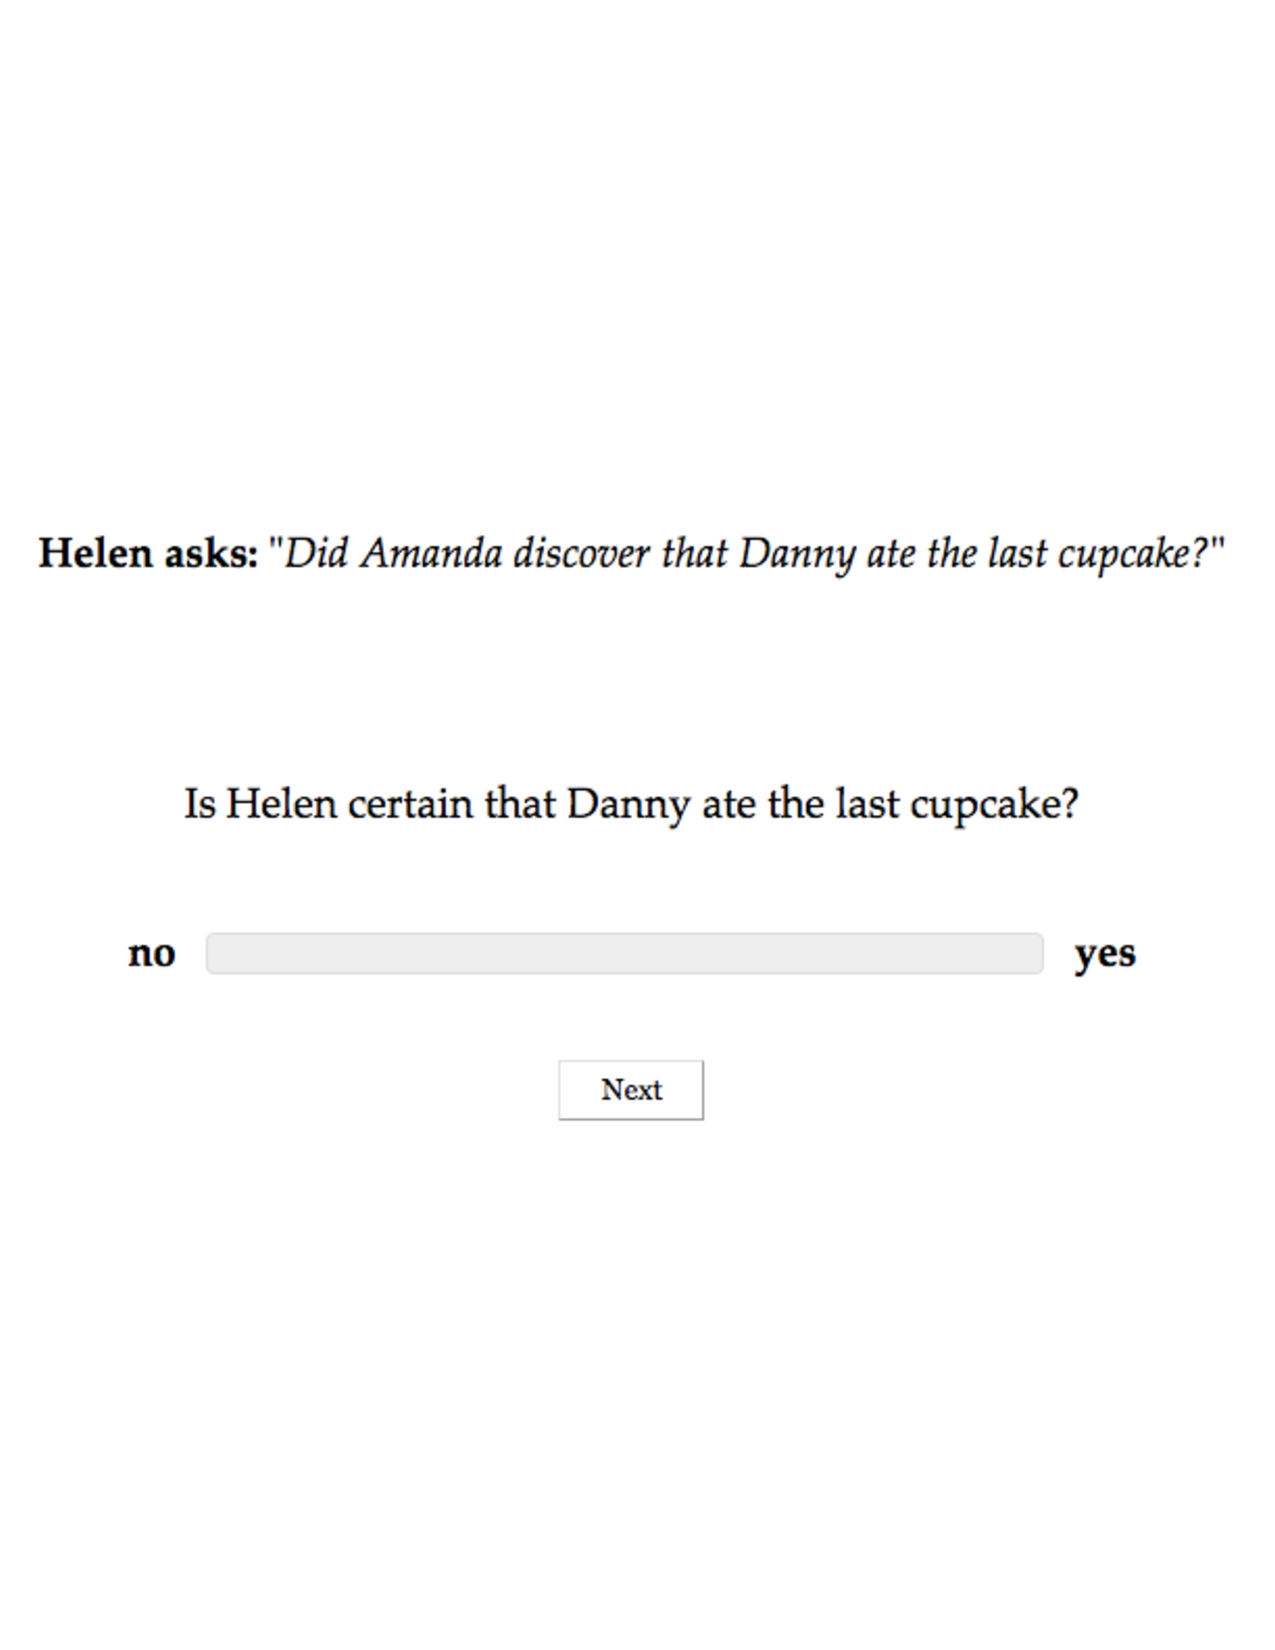
\includegraphics[width=10cm]{figures/trial-exp1}}
\end{center}
\caption{A sample trial in Experiment 1}\label{fig-trial-exp1}
\end{figure}

After completing the experiment, participants filled out a short, optional survey about their age, their gender, their native language(s) and, if English is their native language, whether they are a speaker of American English (as opposed to, e.g., Australian or Indian English). To encourage them to respond truthfully, participants were told that they would be paid no matter what answers they gave in the survey.

\paragraph{Data exclusion}
Prior to analysis, the data from 13 participants who did not self-identify as native speakers of American English were excluded. To assess whether the remaining 287 participants attended to the task, we inspected their responses to the 6 control stimuli, for which we expected low responses. We excluded the data from 16 participants whose response means on the controls were more than 2 standard deviations above the group mean. We furthermore identified 5 participants whose variance in overall response distribution was more than 2 standard deviations below the mean by-participant variance: these participants always selected roughly the same point on the response scale. We excluded the data from these 5 participants, too, leaving data from 266 participants (ages 20-71; median: 36; 118 female, 143 male, 2 other, 3 undeclared).

\subsection{Results and discussion}\label{s22}

Figure \ref{f-projectivity} plots the mean certainty ratings for the target stimuli by predicate, in increasing order from left to right, as well as for the main clause stimuli (abbreviated `MC'). Factive predicates are given in purple, optionally factive predicates in orange, veridical non-factive predicates in blue, and non-veridical non-factive predicates in gray. Participants' individual ratings are given by light gray dots.  The mean certainty ratings are largely consistent with impressionistic judgments reported in the literature: First, the ratings for main clause content are lowest overall, as expected for non-projective content. Second, the ratings for factive predicates are among the highest overall, suggesting comparatively high projectivity of the CC. Third, the mean certainty ratings of many optionally factive predicates are lower than those of many factive predicates and higher than those of main clauses as well as of non-veridical non-factives. However, Figure \ref{f-projectivity} also shows that the CCs of the 5 predicates assumed to be factive are not categorically more projective than the CCs of the optionally factive predicates, contrary to what is expected under the first definition of factive predicates. Specifically, the CCs of the optionally factive predicates {\em acknowledge, hear} and {\em inform} are at least as projective as the CCs of {\em reveal} or {\em discover}. This finding suggests that projectivity alone does not categorically distinguish factive predicates from optionally factive and non-factive ones.

\begin{figure}[H]
\centering

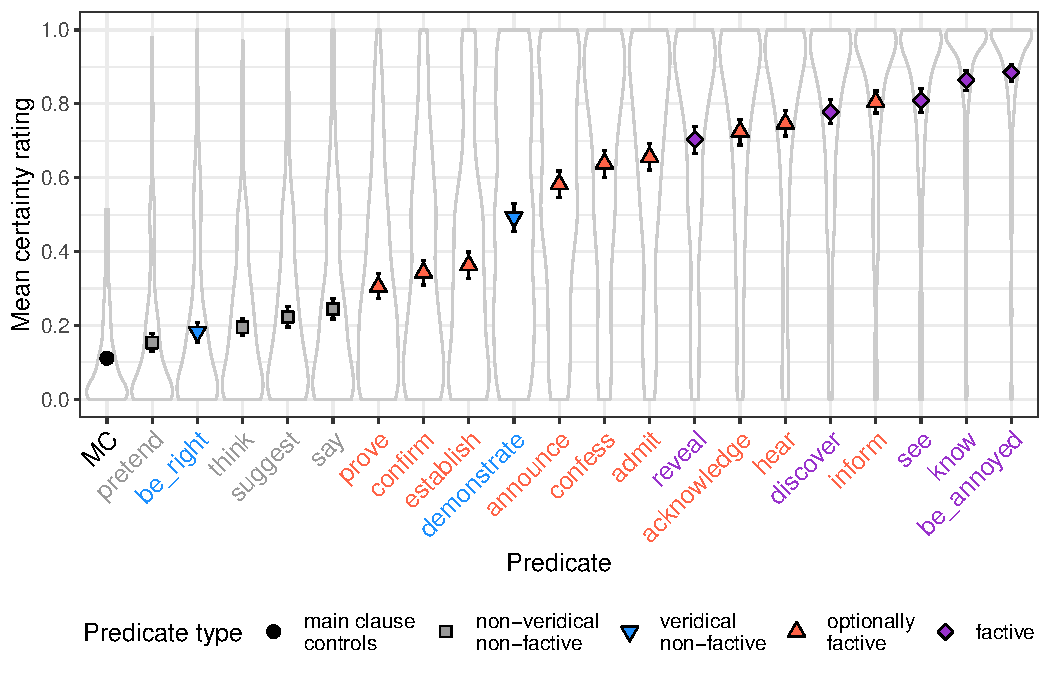
\includegraphics[width=.7\paperwidth]{../../results/5-projectivity-no-fact/graphs/means-projectivity-by-predicate-variability}

\caption{Mean certainty ratings by predicate, collapsing over complement clauses, with 95\% bootstrapped confidence intervals. Factive predicates are given in purple, veridical non-factive ones in blue, non-veridical non-factive ones in gray and optionally factive ones in orange. Light gray dots indicate individual participants' responses. `MC' abbreviates main clause stimuli.}
\label{f-projectivity}
\end{figure}




%1 acknowledge 0.725 0.0330  0.0339  0.692 0.758
% 2 admit       0.656 0.0390  0.0352  0.617 0.691
% 3 announce    0.582 0.0375  0.0370  0.545 0.619
% 4 be_annoyed  0.885 0.0220  0.0226  0.863 0.907
% 5 be_right    0.183 0.0271  0.0251  0.155 0.208
% 6 confess     0.639 0.0399  0.0376  0.599 0.676
% 7 confirm     0.343 0.0350  0.0358  0.308 0.379
% 8 MC          0.111 0.00895 0.00860 0.102 0.120
% 9 demonstrate 0.493 0.0403  0.0382  0.452 0.531
%10 discover    0.779 0.0303  0.0308  0.748 0.809
%11 establish   0.363 0.0340  0.0404  0.329 0.403
%12 hear        0.747 0.0371  0.0360  0.710 0.783
%13 inform      0.805 0.0287  0.0305  0.776 0.836
%14 know        0.864 0.0269  0.0241  0.837 0.888
%15 pretend     0.153 0.0232  0.0276  0.130 0.181
%16 prove       0.305 0.0314  0.0289  0.273 0.334
%17 reveal      0.704 0.0377  0.0349  0.666 0.739
%18 say         0.245 0.0283  0.0287  0.216 0.273
%19 see         0.809 0.0330  0.0303  0.776 0.840
%20 suggest     0.223 0.0256  0.0253  0.197 0.248
%21 think       0.195 0.0236  0.0243  0.172 0.220


One might ask, of course, whether the categorization of clause-embedding predicates assumed in (\ref{pred}) is incorrect and whether there is a different place in which a line can be drawn between factive and optionally factive predicates based on the projectivity of the CCs. The mean certainty ratings plotted in Figure \ref{f-projectivity} suggest that this cannot be done in a non-arbitrary way. For instance, one might consider all predicates as factive whose CC is at least as projective as that of {\em reveal}: this would mean that the predicates typically taken to be factive are factive, as well as {\em acknowledge, hear} and {\em inform}. There is, however, no principled reason why the projectivity of the CC of {\em reveal} should be the cut-off for factivity. It is equally unprincipled to pick an arbitrary mean certainty rating, say .8, and to categorize predicates whose CC has a mean certainty rating of at least .8 as factive and predicates whose CC has a mean certainty rating below .8 as optionally factive. After all, one could just as well pick a threshold of .85 or .75, with the result that different predicates would be considered factive: for instance, {\em discover} (mean: .78) would not count as factive with a threshold of .8, but would with a threshold of .75, and {\em see} (mean: .81) would count as factive with a threshold of .8, but not with a threshold of .85.\footnote{Choosing an arbitrary numeric threshold for factivity is also complicated by the fact that there is by-experiment variation in mean certainty ratings. For instance, the mean certainty ratings in Exp.~1 were lower, overall, than the mean certainty ratings in \citetpos{tbd-variability} Exps.~1. For example, the CC of {\em be annoyed}, which was the most projective in both sets of experiments, received mean certainty ratings of .96  and .92 in \citetpos{tbd-variability} Exps.~1a and 1b, respectively, but only a .86 in our Exp.~1. This difference may be due to the fact that \citet{tbd-variability} primarily investigated highly projective content whereas our Exp.~1 included a wide range of less projective content: it is possible that participants' certainty ratings were influenced by the overall projectivity of the contents investigated. We leave this matter to future research.}

The possibility of categorizing clause-embedding predicates by the projectivity of the CC is further called into question by the fact that the CC of all of the 20 predicates investigated is projective, albeit to varying degrees, compared to the non-projective main clause controls. {\bf Describe models here; also give more general explanation of ZOIB models here.} In other words, speakers who utter an interrogative with one of the 20 clause-embedding predicates are more likely to be taken to be committed to the CC than to the main clause control content.\footnote{According to \citet[1739]{spector-egre2015}, it is not clear whether the CC of {\em say} is projective. Our Exp.~1 findings suggest that it is weakly projective.}    Thus, to distinguish factive predicates from optionally factive and non-factive ones in this set of 20 predicates, one would need to distinguish one group of projective CCs from another group of projective CCs. We propose that there is no principled way of doing so.

One might also wonder whether a different projectivity diagnostic might result in a categorical distinction between factive predicates, on the one hand, and optionally factive and non-factive ones, on the other. For instance, one might wonder whether a categorical distinction emerges if binary certainty ratings are collected, that is, if participants are forced to identify whether or not the speaker is certain of the relevant content. To assess this possibility, we ran a follow-up experiment that was identical to Exp.~1, except that we used a two-alternative forced choice task; that is, participants were asked to respond `yes' (coded as 1) or `no' (coded as 0) to the question of whether the speaker is certain of the relevant content (see Appendix \ref{a-binary} for details). We refer to this experiment as Exp.~1$'$. Figure \ref{f-projectivity2} plots the proportion of `yes' ratings (indicating projection) by predicate, again in increasing order from left to right, as well as the ratings for the main clause stimuli (again abbreviated `MC'). Jittered gray dots indicate the 426 individual participants' ratings. The findings of Exp.~1$'$ are strikingly similar to those of Exp.~1, as evidenced by the very high Spearman rank correlation of .983 (for a figure, see Appendix \ref{a-binary}),\footnote{The Spearman rank correlation coefficient, a value between -1 and 1, is a nonparametric measure of rank correlation: the higher the coefficient, the more the relation between the dependent and the independent variables can be described using a monotonic function; if the coefficient is positive, the value of the dependent variable tends to increase with an increase in the independent variable. In the case of our experiments, a coefficient of 1 would mean that there is a perfectly monotone increasing relation between the ranking of the predicates in Exp.~1 and Exp.~1$'$: for any two predicates $p_1$ and $p_2$, if $p_1$ ranks below $p_2$ in Exp.~1 (that is, the mean certainty rating of $p_1$ is lower than that of $p_2$), then that ranking is preserved in Exp.~1$'$.} and the critical findings of Exp.~1 were replicated. First, the CCs of the factive predicates are not categorically more projective than the CCs of the optionally factive predicates:  the CCs of {\em acknowledge, hear} and {\em inform} are at least as projective as the CCs of {\em reveal} or {\em discover}. Second, a non-arbitrary line between factive and optionally factive predicates cannot be drawn, as the CC of all factive and optionally factive predicates are projective compared to the non-projective main clause controls.\footnote{Compared to the projectivity of the CC of {\em be right}, which were the least projective of all CCs, the CCs of the other 19 predicates were more projective. {\bf Describe model here, explain why we couldn't use the main clause controls as reference level: no variance.}}  Thus, the findings of Exp.~1$'$ also do not support the assumption that factive predicates are categorically distinguished from optionally factive and non-factive ones by the projectivity of the CC alone. 

\begin{figure}[H]

\centering
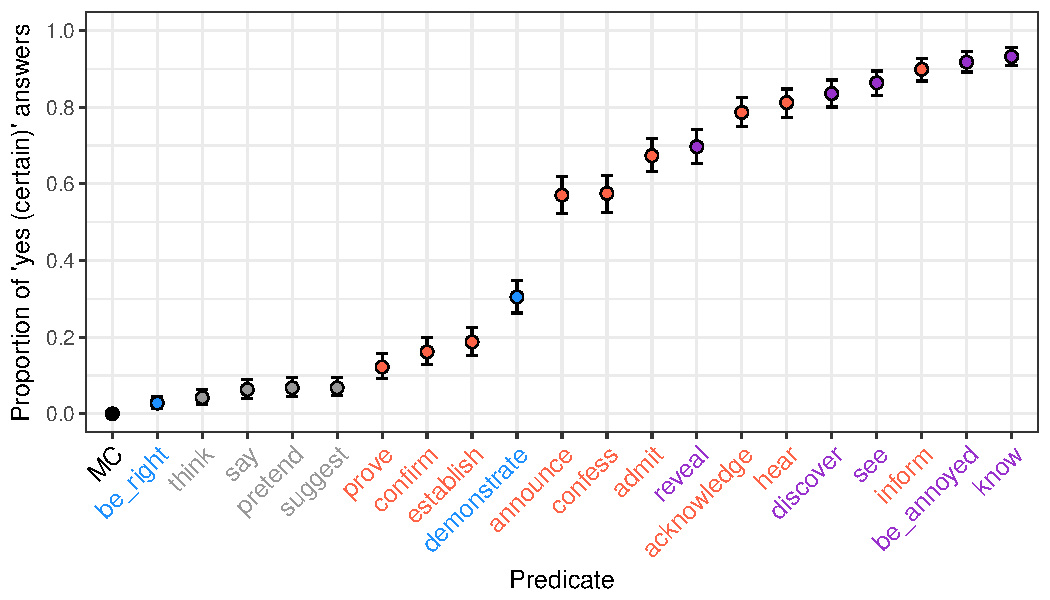
\includegraphics[width=.7\paperwidth]{../../results/8-projectivity-no-fact-binary/graphs/proportion-by-predicate-variability}
\caption{Proportion of `yes' ratings by predicate, collapsing over complement clauses, with 95\% bootstrapped confidence intervals. Factive predicates are given in purple, veridical non-factive ones in blue, non-veridical non-factive ones in gray and optionally factive ones in orange. `MC' abbreviates main clause.}\label{f-projectivity2}

\end{figure}

Converging evidence for our finding comes from two additional datasets. First, \citet*{demarneffe-etal-sub23} found that factive predicates do not receive categorically higher mean certainty ratings than optionally factive predicates in the CommitmentBank, a collection of naturally occurring discourses with clause-embedding predicates embedded under a variety of entailment-canceling operators. A second piece of converging evidence comes from the MegaVeridicality dataset (\citealt{white-rawlins-nels2018,white-etal2018b}),\footnote{This dataset is  available at \url{http://megaattitude.io.}. The R code of our analysis of the data can be found at  [redacted for review].}
%\url{https://github.com/judith-tonhauser/factivity}.}   
which contains projectivity ratings for the CCs of 517 English clause-embedding predicates. The stimuli that participants rated consisted of combinations of the 517 predicates with arguments with low lexical content, as shown in (\ref{wr-stim-proj}) for the predicate {\em know}: the predicates and their clausal complements were embedded under negation in stimuli like (\ref{wr-stim-proj}a) and under both negation and the question operator in stimuli like (\ref{wr-stim-proj}b). To assess projectivity, participants were asked to respond to the question {\em Did that thing happen?} for stimuli like (\ref{wr-stim-proj}a) and to respond to the question posed by stimuli like (\ref{wr-stim-proj}b). The response options were `yes', `maybe or maybe not' and `no'. 

\begin{exe}
\ex\label{wr-stim-proj}
\begin{xlist}
\ex Somebody didn't know that a particular thing happened.
\ex If somebody didn't know that a particular thing happened, did that thing happen?
\end{xlist}
\end{exe}

Each of the 517 predicates in the MegaVeridicality dataset received between 29 and 60 projectivity ratings (mean: 32) from a total of 290 participants. To plot the ratings and to compare them to the findings of our experiments, we coded a `yes' response as 1,  a `maybe or maybe not' response as 0 and a `no' response as -1.\footnote{We assume that a `maybe or maybe not' response means that the participant is not certain whether the CC is true (i.e., whether that thing happened) and that a `no' response means that the CC is false (i.e., that thing did not happen). Thus, for ease of comparison with our data, a `maybe or maybe not' response was coded as 0.} Figure \ref{f-white-rawlins-projectivity} plots the mean projectivity ratings for the 517 predicates in the MegaVeridicality dataset, with x-axis labels for 19 of the 20 predicates that we investigated (the predicate {\em be right} is not part of the MegaVeridicality dataset). As shown,\footnote{The x-axis labels for the following predicates overlap: {\em discover/confirm} and {\em acknowledge/say/admit}.} projectivity does not categorically distinguish factive predicates from optionally factive and non-factive ones: the CCs of the optionally factive predicates {\em confess, acknowledge, announce, hear} and {\em inform} are at least as projective as those of some factive predicates. Thus, the MegaVeridicality dataset confirms our finding, that projectivity alone does not categorically distinguish factive predicates from optionally factive and non-factive ones, contrary to what we expect under the first definition of factive predicates.

\begin{figure}[H]
\centering
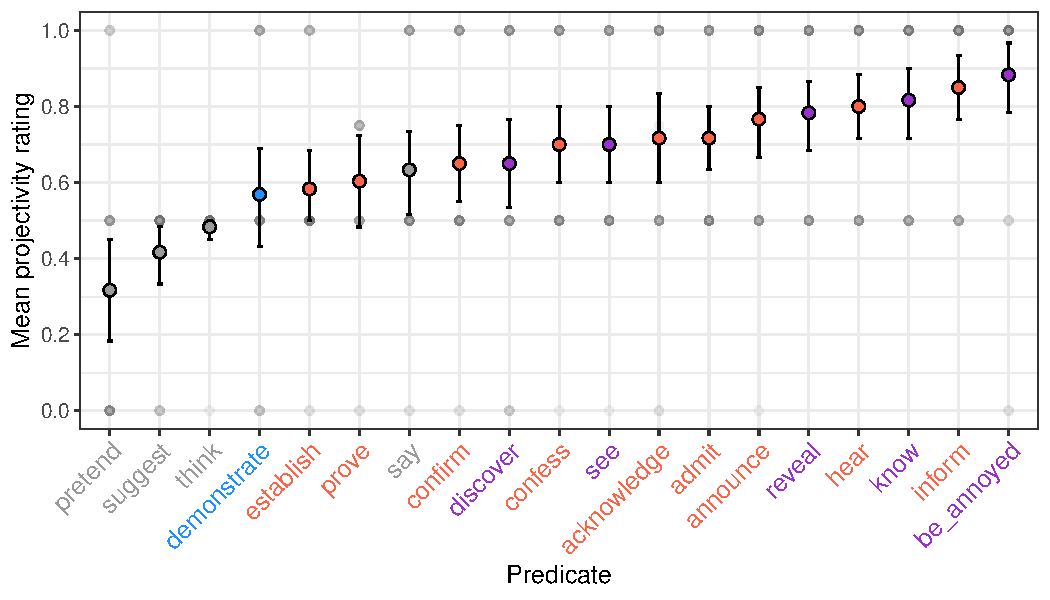
\includegraphics[width=.75\paperwidth]{../../white-rawlins-data/graphs/means-projection-by-predicate}

\caption{Mean projectivity rating in blue, by predicate, with 95\% bootstrapped confidence intervals, for the 517 predicates in MegaVeridicality dataset. X-axis labels for 19 of the 20 predicates featured in our Exps.~1 and 2: factive predicates in purple, the veridical non-factive one in blue, non-veridical non-factive ones in gray and optionally factive ones in orange.}
\label{f-white-rawlins-projectivity}
\end{figure}

While we cannot, of course, rule out the possibility that a different projectivity diagnostic may categorically distinguish factive predicates from optionally factive and non-factive ones, we suggest that projectivity alone does not result in such a distinction, contrary to what the first definition of factive predicates leads us to expect. The experiments described in the next section were designed to explore whether the CC of the same 20 predicates is entailed, to identify whether entailment and projectivity jointly categorize clause-embedding predicates, as per the second definition of factive predicates.

 
\section{Experiment}\label{s3}

\section{Discussion}

\section{Conclusions}

\appendix

\setcounter{table}{0}
\renewcommand{\thetable}{A\arabic{table}}

\setcounter{figure}{0}
\renewcommand{\thefigure}{A\arabic{figure}}

\section{20 complement clauses}\label{a-clauses}

The following clauses realized the complements of the predicates in the three experiments: 

\begin{enumerate}[leftmargin=3ex,itemsep=-2pt]

\begin{multicols}{2}

\item Mary is pregnant.
\item Josie went on vacation to France.
\item Emma studied on Saturday morning.
\item Olivia sleeps until noon.
\item Sophia got a tattoo.
\item Mia drank 2 cocktails last night.
\item Isabella ate a steak on Sunday.
\item  Emily bought a car yesterday.
\item  Grace visited her sister.
\item Zoe calculated the tip.

\columnbreak

\item  Danny ate the last cupcake.
\item  Frank got a cat.
\item  Jackson ran 10 miles.
\item  Jayden rented a car.
\item  Tony had a drink last night.
\item  Josh learned to ride a bike yesterday.
\item  Owen shoveled snow last winter.
\item  Julian dances salsa.
\item  Jon walks to work.
\item  Charley speaks Spanish.

\end{multicols}

\end{enumerate}

\bibliographystyle{/Users/tonhauser.1/Library/Latex/cslipubs-natbib}
\bibliography{/Users/tonhauser.1/Documents/bibliography}

\end{document}

